% Notes:
% - The point that central regions of low J_z, density flattens = no constraining power
% - The condition on d(r_z)/d(r_z')
% - Widmark papers
% - https://arxiv.org/abs/2303.18040

% \begin{figure}[!t]
% \begin{center}
% % \includegraphics[width=0.9\textwidth]{visitstats.pdf}
% {\color{red} Figure placeholder}
% \end{center}
% \caption{%
% TODO
% \label{fig:chiplots}
% }
% \end{figure}

\PassOptionsToPackage{usenames,dvipsnames}{xcolor}
\documentclass[modern]{aastex631}
% \documentclass[twocolumn]{aastex631}

% Load common packages
\usepackage{microtype}  % ALWAYS!
\usepackage{amsmath}
\usepackage{amsfonts}
\usepackage{amssymb}
\usepackage{booktabs}
\usepackage{graphicx}
% \usepackage{color}

\usepackage{enumitem}
\setlist[description]{style=unboxed}

% Some style hacks:
\renewcommand{\twocolumngrid}{\onecolumngrid}
\setlength{\parindent}{1.1\baselineskip}
\addtolength{\topmargin}{-0.2in}
\addtolength{\textheight}{0.4in}
\sloppy\sloppypar\raggedbottom\frenchspacing

\graphicspath{{figures/}}
% \definecolor{cbblue}{HTML}{3182bd}
% \usepackage{hyperref}
% \definecolor{linkcolor}{rgb}{0.02,0.35,0.55}
% \definecolor{citecolor}{rgb}{0.45,0.45,0.45}
% \hypersetup{colorlinks=true,linkcolor=linkcolor,citecolor=citecolor,
%             filecolor=linkcolor,urlcolor=linkcolor}
% \hypersetup{pageanchor=true}

\newcommand{\documentname}{\textsl{Article}}
\newcommand{\sectionname}{Section}
\renewcommand{\figurename}{Figure}
\newcommand{\equationname}{Equation}
\renewcommand{\tablename}{Table}

% Missions
\newcommand{\project}[1]{\textsl{#1}}

% Packages / projects / programming
\newcommand{\package}[1]{\textsl{#1}}
\newcommand{\acronym}[1]{{\small{#1}}}
\newcommand{\github}{\package{GitHub}}
\newcommand{\python}{\package{Python}}
\newcommand{\jax}{\package{JAX}}
\newcommand{\emcee}{\project{emcee}}

% Stats / probability
\newcommand{\given}{\,|\,}
\newcommand{\norm}{\mathcal{N}}
\newcommand{\pdf}{\textsl{pdf}}

% Maths
\newcommand{\dd}{\mathrm{d}}
\newcommand{\deriv}[2]{\frac{\mathrm{d}{#1}}{\mathrm{d}{#2}}}
\newcommand{\dderiv}[2]{\frac{\mathrm{d^2}{#1}}{\mathrm{d}{#2}^2}}
\newcommand{\Deriv}[2]{\frac{\mathrm{D}{#1}}{\mathrm{D}{#2}}}
\newcommand{\pderiv}[2]{\frac{\partial {#1}}{\partial {#2}}}
\newcommand{\ppderiv}[2]{\frac{\partial^2 {#1}}{\partial {#2}^2}}
\newcommand{\transpose}[1]{{#1}^{\mathsf{T}}}
\newcommand{\inverse}[1]{{#1}^{-1}}
\newcommand{\argmin}{\operatornamewithlimits{argmin}}
\newcommand{\mean}[1]{\left< #1 \right>}

% Non-scalar variables
\renewcommand{\vec}[1]{\ensuremath{\bs{#1}}}
\newcommand{\mat}[1]{\ensuremath{\mathbf{#1}}}

% Units:
% Workaround for siunitx + AASTeX
% https://tex.stackexchange.com/questions/192610/use-emulateapj-aastex-with-siunitx
\usepackage{savesym}
\savesymbol{tablenum}
\usepackage{siunitx}
\restoresymbol{SIX}{tablenum}
\DeclareSIUnit\year{yr}
\DeclareSIUnit\parsec{pc}
\DeclareSIUnit\Msun{M_\odot}
\DeclareSIUnit\Rsun{R_\odot}
\newcommand{\mas}{\unit{\milli\arcsecond}}
\newcommand{\muas}{\unit{\micro\arcsecond}}
\newcommand{\kms}{\unit{\km\per\s}}
\newcommand{\kpc}{\unit{\kilo\parsec}}



% Misc.
\newcommand{\bs}[1]{\boldsymbol{#1}}

% Astronomy
\newcommand{\DM}{{\rm DM}}
\newcommand{\feh}{\ensuremath{{[{\rm Fe}/{\rm H}]}}}
\newcommand{\mh}{\ensuremath{{[{\rm M}/{\rm H}]}}}
\newcommand{\logg}{\ensuremath{\log g}}
\newcommand{\Teff}{\ensuremath{T_{\textrm{eff}}}}
\newcommand{\vsini}{\ensuremath{v\,\sin i}}
\newcommand{\mtwomin}{\ensuremath{M_{2, {\rm min}}}}

% Dynamics
\newcommand{\df}{\acronym{DF}}

% TO DO
\newcommand{\todo}[1]{{\color{red} TODO: #1}}
\newcommand{\placeholder}[1]{{\color{purple} #1}}

\newcommand{\gaia}{\textsl{Gaia}}
\newcommand{\dr}[1]{\acronym{DR}#1}
\newcommand{\apogee}{\acronym{APOGEE}}
\newcommand{\sdss}{\acronym{SDSS}}
\newcommand{\sdssiv}{\acronym{SDSS-IV}}
\newcommand{\thejoker}{\project{The~Joker}}


\shorttitle{}
\shortauthors{Price-Whelan et al.}

\begin{document}

\title{
    Data-driven Dynamics with Orbital Torus Imaging:  \\
    A Flexible Model of the Vertical Phase-space of the Galaxy
}
% ChatGPT: Empirical Modeling of Vertical Phase-Space Density in the Milky Way: A Flexible Method for Inferring the Acceleration Field

\newcommand{\affcca}{
    Center for Computational Astrophysics, Flatiron Institute, \\
    162 Fifth Ave, New York, NY 10010, USA
}

\author[0000-0003-0872-7098]{Adrian~M.~Price-Whelan}
\affiliation{\affcca}
\email{aprice-whelan@flatironinstitute.org}
\correspondingauthor{Adrian M. Price-Whelan}

\author{Jason A. S. Hunt}
\affiliation{\affcca}

\author{Daniel~Horta~Darrington}
\affiliation{\affcca}

\author{Kathryn Johnston}
% \affiliation{\affcolumbia}

% TODO: orcid, affs
\author{David~W.~Hogg}
% \affiliation{\affcca}
% \affiliation{\affnyu}
% \affiliation{\affmpia}

\author{Lawrence Widrow}

\author{Benjamin~Cassese}

\author{Neige Frankel}

\author{+ more, ORDER TBD!}


\begin{abstract}\noindent
\emph{Old abstract - needs rethinking}
% Context
In a steady-state dynamical system, spatial gradients of the phase-space density (the
distribution function, \df) of any tracers are related to gradients of the underlying
gravitational potential (the acceleration field).
This is the basis of many methods used in Galactic dynamics to infer the mass or dark
matter distribution of the Milky Way, often with highly-symmetric, few-component,
parametric models of the Galaxy (e.g., an exponential disk with constant scale height).
However, we know that the Galaxy is not in equilibrium and its mass distribution is
complex:
Stellar kinematics show signatures of non-steady-state dynamics throughout the Galactic
disk and significant departures from axisymmetry.
% Aims
We aim to develop a framework for measuring the acceleration field of the Milky Way, in
the presence of weak disequilibrium, that makes few assumptions about the form of the
mass distribution.
% Methods
Here we outline a flexible method for empirically modeling the vertical phase-space
density (or mean statistics of stellar invariants in this phase-space, like element
abundances) of stars in the Galactic disk.
This method --- an improved version of the method of \emph{Orbital Torus Imaging} (OTI)
--- works by exploiting the fact that orbital trajectories in the vertical phase-space
of an unperturbed galaxy have predictable symmetries in projections of phase-space and
can be represented as a low-order Fourier expansion away from an ellipse.
% Results
We first demonstrate OTI using a toy simulation of a vertical phase-space distribution
of stars, then with a more realistic galactic disk population, and show that in both
cases OTI recovers the local vertical acceleration as a function of height above the
galactic midplane.
We then show that this method enables us to compute \emph{empirical} orbital actions,
angles, and frequencies for stars where the approximation of a separable 1D phase-space
is valid: This enables interpreting the timescales of disequilibrium features in a
flexible way that does not require adopting a global model of the gravitational
potential.
For example, we demonstrate that this method provides a useful tool for studying the
\emph{residuals} away from an equilibrium model, such as the ``\gaia\ Phase Spiral.''
% Conclusions
Some conclusions.

% Context
% Orbital dynamics is complex in six-dimensional phase-space, making it a challenge to
% interpret the rich and structured kinematic data of stars in the Milky Way revealed in
% recent data releases from the \gaia\ Mission.
% In a symmetric, steady-state galaxy, or in the presence of only weak perturbations, the
% dynamical interpretation and investigation of kinematic data is often simplified by
% using dynamical invariants such as orbital actions.
% However, computing many such quantities (e.g., the energy, actions, fundamental
% frequencies, etc.) require having a model for the gravitational potential and, even so,
% are either slow to compute or imprecise.
% % Aims
% To mitigate at least one of these limitations, we aim to demonstrate a method for
% estimating fundamental galactic orbital properties for stars directly from the kinematic
% and stellar label data (e.g., element abundances) without requiring a gravitational
% potential model.
% % Methods
% This method still assumes a symmetric and steady-state distribution function, but uses
% either the number density of stars in a slice of phase-space (e.g., vertical $z$--$v_z$
% kinematics) or a statistic computed from other stellar invariants in this slice (e.g.,
% element abundances) to empirically estimate orbital actions, frequencies, and angles for
% the stars.
% % Results
% We demonstrate the method using a toy equilibrium model where orbital properties are
% known, and then show applications of this method even in the presence of disequilibrium.
% As a last demonstration, we use data from the \gaia\ Mission to estimate the total mass
% density at the Galactic midplane as a function of radius near the sun.
% % Conclusions
% We conclude :shrugs:.

\end{abstract}

% \keywords{}

\section{Introduction} \label{sec:intro}

Measuring and studying the mass distribution of the Milky Way is an important venture
for many applications in astrophysics.
For one, the total mass distribution determines the orbits of its gas, stars, star
clusters, and satellite galaxies, and thus enables interpreting the kinematic snapshot
we observe in terms of dynamical and galactic evolutionary processes.
The Galactic mass distribution also encodes the structure of dark matter around the
Milky Way, which provides an important laboratory for studying the astrophysical
properties of dark matter on the scale of an individual galaxy.
On these mass scales (and smaller), effective models for dark matter predict different
radial density profiles and different populations of substructure.
It is therefore hoped that precise measurements of the structure of dark matter within
the Milky Way and other nearby galaxies will enable new constraints on the particle
nature of dark matter.

Until direct measurements of the Galactic acceleration field become more ubiquitous, our
best hope for studying the acceleration field of the Milky Way (and therefore its mass
distribution and dark matter content) comes from modeling stellar kinematics.
The principle challenge of this problem is that we only observe a \emph{snapshot} of the
kinematics (i.e. positions $\bs{x}$ and velocities $\bs{v}$) and other stellar
properties (i.e. element abundances, ages, etc.) of tracer populations throughout the
Galaxy at present day.
In order to relate this kinematic snapshot of tracers to the acceleration field, there
are two main limits that dictate what methods one can use: (1) the phase-mixed and
equilibrium case, and (2) the phase-coherent case.
When a stellar system is in equilibrium and the distribution function (DF, $f(\bs{x},
\bs{v})$) is in steady state, the DF can be expressed as a function of only integrals of
motion (e.g., the orbital actions, $\bs{J}$, so that $f(\bs{J})$).
This enables using a number of dynamical inference methods that either try to explicitly
model the DF (e.g., ``DF modelling'' methods), its derivatives (e.g., the Collisionless
Boltzmann Equation), or moments of the DF (e.g., the Jeans equations).
- Used for decades, but can be a challenge because historically censored or modified by
survey selection effects, and historically we only had access to subsets of the full set
of phase-space coordinates $(\bs{x}, \bs{v})$.
- Often the gravitational potential $\Phi$ is additionally assumed to be highly
symmetric and is represented using simple analytic mass models (i.e. a sum of a
spherical dark matter component, a component to represent the Galactic bulge, plus an
axisymmetric disk component; see, e.g., \citealt{TODO}), and the tracer DF is explicitly
parametrized \citep[e.g.,][]{TODO}.

In the phase-coherent case, the DF is not in steady state and therefore could depend
explicitly on time and orbital phase (e.g., the orbital angles $\bs{\theta}$).
- When the DF depends strongly on angles, there are no generic methods ... case-by-case.
- For example, stellar streams tell us about orbits and more directly about acceleration. Can be more powerful than equilibrium methods.

- MW disk is probably somewhere in between
- Old enough to have erased much of its initial conditions
- But interacting with satellites and internal non-equilibrium processes keep it out of equilibrium/steady-state
- Shown clearly be recent data ... phase spiral yadda yadda
This research direction has been revolutionized by recent data releases from the \gaia\
Mission \citep{TODO}.
- This means generically, methods that assume equilibrium will be biased
- But still useful because subtracting equilibrium models can reveal non-equilibrium structure

- Transition to discussing how we have access to way more information
- and larger stellar spectroscopic surveys of the Galaxy \citep{APOGEE, GALAH, RAVE, LAMOST, TODO}



For one, \gaia\ has given us access to stellar kinematic measurements for a large number
of stars over a substantial volume of the Milky Way, enabling an almost direct (modulo
selection effects from the survey and Galactic extinction) reconstruction of the stellar
tracer DF $f$.
- Revitalized approaches that explicitly model the DF, not moments
With models or reconstructions of the tracer DF, one can either use the CBE (or Jeans
equations) to directly estimate the vertical acceleration field under all of the
assumptions discussed above \citep{greggreen, jatanbuch, TODO}, or construct an
action-based model (a so-called ``$f(J)$'' model) in which the potential constraining
power comes from the implicit transformation to action-angle coordinates \citep{sanders,
others}.

The impressive precision of the \gaia\ data has also been transformative for revealing
intricate substructure in the DF that was previously seen at low significance or
unknown.
For example, \gaia\ has revealed a ``phase spiral'' in the vertical kinematics of stars
in the Galactic disk \citep[e.g.,][]{Antoja, many, TODO}, has enabled mapping the bulk,
in-plane kinematics of stars in the disk \citep[e.g.,][]{Katz, Eilers, TODO}, and has
enabled quantifying the stellar warp and structure of the outer Milky Way disk
\citep[e.g.,][]{Poggio, Antoja, TODO}.
Given the complexity apparent in the observed DF of the Milky Way, it is increasingly
important to develop new modeling methods that can account for disequilibrium, and to
use new kinds of data to help interpret and characterize the Milky Way's acceleration
field.

Spectroscopic surveys open up new dimensions.
Add radial velocities for distant stars, but also element abundances.
Element abundances and stellar parameters are complementary to phase-space invariants.
Can be used to study dynamical state of disk by combining with kinematic quantities.
Mono-abundance populations (MAPs): $p(\bs{J} \given \bs{X})$ (Bovy)
DF modeling: $p(\bs{J} \given \bs{X})$ (Sanders)
We introduced the idea of Orbital Torus Imaging: $p(\bs{X} \given \bs{J})$ (PW21).

OTI is the idea that ...
Conditioned on action, so less sensitive to survey selection effects and dust.
Uses the abundances to help constrain the dynamics.

Advances in data motivate advances in methods, and using new kinds of data.
This work defines a new approach for studying the Milky Way's acceleration field using
stellar invariants or the phase-space density, in the spirit of OTI.
Potential to go to multiple dimensions and non-equilibrium phase structure, but here we
start with 1D and equilibrium models (still useful to look at residuals).

Another use case for modeling the phase-space density or the dependence of other stellar
invariants is to assess the level of asymmetric or non-equilibrium structure in the
Galaxy.


\section{Method} \label{sec:method}

% Notes:
% - We measure the DF, so can take gradients, but to get to acceleration and potential,
%   we need to know df/dt.

Figure 1: Show that contours of DF = orbits
Figure 2: rz' vs. thetaz' for a few different orbits - show that m=2, m=4??
Figure 3: Test on simple case: isothermal or SHO, simple?? Can recover actions, frequencies, etc.
Figure 4: Real galaxy - not separable. Agama equilibrium model. Still does well!
Figure 5:



In a collisionless system, the distribution function of stellar kinematics,
$f(\boldsymbol{x}, \boldsymbol{v}, t)$, is a fundamental ...

Separability
CBE

Our goal is to model the stellar phase-space density
$f(\boldsymbol{x}, \boldsymbol{v})$, or the functional dependence of statistics computed
from stellar invariants for stars on different orbits $X(\boldsymbol{x},
\boldsymbol{v})$, as a means toward

From this model, we can then measure the acceleration field from gradients of the DF, can determine the mean density field from frequencies.

to both (1) infer the local acceleration field, and (2) determine a local, empirical transformation to actions, angles, and frequencies

to infer a local transformation to actions, angles,
and frequencies without assuming a particular model for the gravitational potential of
the Galaxy.
As motivation and context, we presume that we have access to precise and accurate
measurements of the stellar positions and velocities $(\bs{x}, \bs{v})$ for a large
sample of stars in the Milky Way (for example, from the \gaia\ Mission; \citealt{TODO}).
Conceptually, our plan is to infer a flexible model of the local phase-space
distribution function (DF), $f(\bs{x}, \bs{v})$, and use levels of constant phase-space
density (or constant stellar invariants) to trace the shapes of orbits in phase space.


\subsection{Setup and Assumptions} \label{sec:methods-setup}

For simplicity, in this work we restrict our focus to one-dimensional (1D) kinematics in
the vertical Galactic phase space $(z, v_z)$ (we discuss generalizations of the method
later in the Discussion, Section~\ref{sec:discussion}). % TODO: do this
However, even in a simple, axisymmetric galaxy mass model, stellar orbits are not
separable in cylindrical coordinates $R, z$, meaning that the trajectory a typical star
traces out in the 4D phase-space is coupled in terms of the radial $R$ and vertical $z$
components of motion.
We therefore ... conditional on $J_R=0$


To do this, we make several assumptions or choices to simplify the problem:
\begin{description}
    \item[Axisymmetry] The true gravitational potential that the stars orbit in is
    axisymmetric and smooth (but note that we do not assume a form for this potential).
    \item[1D phase-space / vertical kinematics] Here we focus on vertical position and
    velocity $z, v_z$, but this method could equally be applied to the radial kinematics
    $R, v_R$.
    % TODO: here
    \item[Circular orbits] For the previous assumption to be a valid simplification, we
    also require that stars have negligible eccentricity (or zero radial action $J_R=0$)
    and have the same $z$-component of the angular momentum $L_z$ (or azimuthal action
    $J_\phi$).
    \item[Phase-mixed] The stellar distribution function (\df) in any vertical slice of
    the full phase-space is phase-mixed.
    \item[No interactions] The stars do not interact with one another and act
    effectively as test particles orbiting within the galactic mass distribution.
    % TODO: note the assumptions above mean we are working at many R's to have J_R=0 but
    % constant L_z
\end{description}
Under these assumptions --- and importantly in a slice of phase-space at fixed values of
the other actions --- contours of fixed phase-space density (or of fixed stellar
invariant statistics, like stellar abundances; \citealt{Price-Whelan:2021}) delineate
orbital trajectories.
% Argument is: E = 1/2 v_z^2 + Phi(z) -> v_z(z) is an orbit, so f(E) = const. -> v_z(z)
% is also an orbit
This motivates a conceptual path toward empirically determining dynamical quantities of
interest directly from the observed phase-space density or from statistics of stellar
labels computed in a slice of phase-space.
% TODO: figure 1 should be referenced here

\begin{figure*}[t!]
\begin{center}
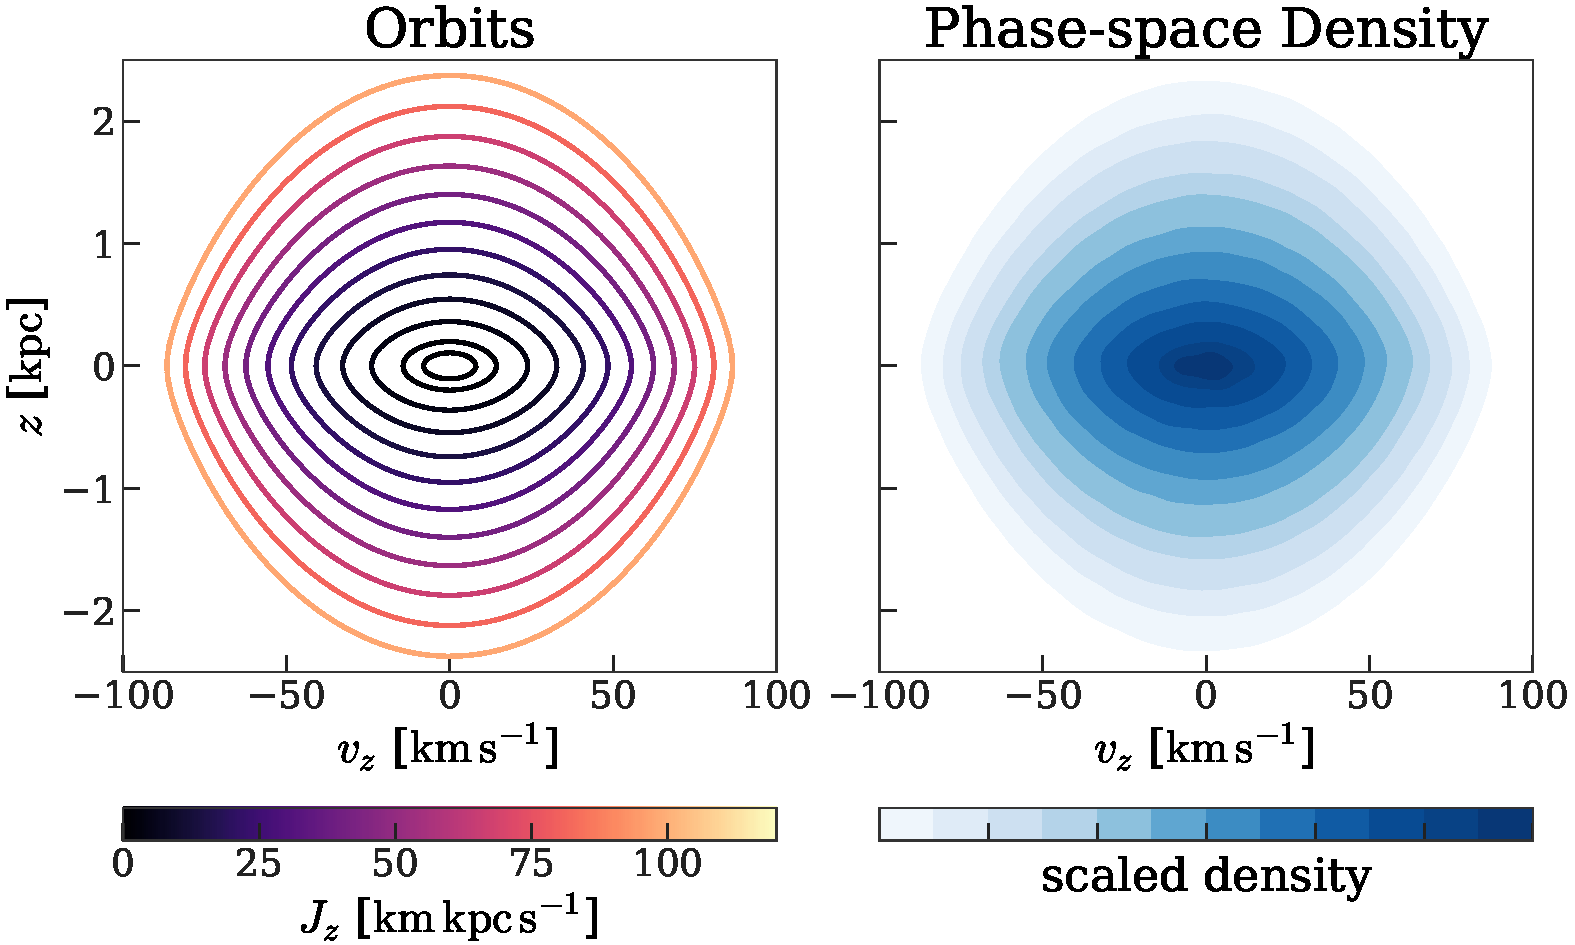
\includegraphics[width=\textwidth]{illustrate-zvz.pdf}
\end{center}
\caption{%
TODO
\label{fig:zvz}
}
\end{figure*}

Given a closed orbital trajectory in a 1D phase-space, we can estimate dynamical
quantities like the orbital actions, angles, and frequencies.
For example, in terms of the vertical position and velocity $z, v_z$, where an orbit can
be parametrized as $v_z(z)$, the vertical action $J_z$ and period $T_z$ are given by
\begin{align}
    J_z &= \frac{2}{\pi} \, \int_0^{z_{\textrm{max}}} \dd z \, v_z(z) \\
    T_z &= 4 \, \int_0^{z_{\textrm{max}}} \frac{\dd z}{v_z(z)}\quad ,
\end{align}
which can then be used to compute the vertical (angular) frequency $\Omega_z =
\frac{2\pi}{T_z}$.
For a given stellar position and velocity $z, v_z$ along an orbit, the vertical angle
$\theta_z$ can be computed as the fraction of an orbital period traversed up to that
point,
\begin{equation}
    \theta_z = \frac{2\pi}{T_z} \, \int_0^{z} \frac{\dd w}{v_z(w)} \quad ,
\end{equation}
where $w$ is an integration variable.
In principle, with infinite particle resolution, one could extract contours of constant
density (or stellar labels) from an observed phase-space distribution and numerically
estimate the integrals above.
In practice, however, this would be noisy and unstable in regions of low phase-space
density, which are often the most interesting (e.g., the transition from disk-dominated
to halo-dominated kinematics).
Instead, in what follows we outline a method for modeling the continuous phase-space
density that enables computing the dynamical quantities.


\subsection{Estimating Dynamical Quantities from the Phase-space Density}

Given a distribution of $N$ stellar positions and velocities $\{z, v_z\}_N$, our task is
to infer the parameters of a functional model for the number density $n(z, v_z)$ that
also allows use to compute the dynamical quantities ($J_z$, $\Omega_z$, $\theta_z$) for
any individual $z, v_z$.
With our assumption that the \df\ is phase-mixed, the number density should only depend
on the phase-space coordinates through the action, so that $n(z, v_z) = n(J_z(z, v_z))$
At fixed $z$, say $z=0$, we expect that $J_z$ increases with increasing $v_z$ (orbits
with larger velocity at the midplane will reach larger heights) and $\Omega_z$
decreases with increasing $v_z$ (orbits that reach larger heights above the midplane
have longer periods).
Similar arguments can be made at fixed $v_z=0$ in considering how $J_z$ and $\Omega_z$
vary with increasing $z$.
It is therefore useful to construct an ellipsoidal polar coordinate system in the $z,
v_z$ plane with a radius coordinate $r_z'$ and a corresponding angle coordinates
$\theta_z'$ defined as
\begin{align}
    r_z' &= \sqrt{z^2 \, \omega_0 + v_z^2 \, \omega_0^{-1}} \label{eq:rzp} \\
    \theta_z' &= \tan^{-1}\left(\frac{z}{v_z}\,\omega_0\right) \label{eq:thetazp}
\end{align}
where $\omega_0$ is a scale frequency.
The vertical action $J_z$ and frequency $\Omega_z$ should be close to monotonic
functions of this polar radius $r_z'$.

For example, in a simple harmonic oscillator (SHO) potential,
\begin{equation}
    \Phi(z) = \frac{1}{2} \, \omega^2 \, z^2
\end{equation}
the Hamiltonian (total energy per unit mass) is
\begin{equation}
    H(z, v_z) = E_z = \frac{1}{2} \, v_z^2 + \frac{1}{2} \, \omega^2 \,z^2
\end{equation}
and the orbital action $J_z$ is given by
\begin{equation}
    J_z = \frac{E_z}{\omega} \quad .
\end{equation}
All orbits have the same frequency $\omega$ and are elliptical in the 1D phase-space.
In this case, the scale frequency $\omega_0$ in $r_z'$ corresponds to the frequency of
the oscillator $\omega_0=\omega$, the radius $r_z'$ is related to the action $J_z$ as
\begin{equation}
    J_z = \frac{1}{2} r_z'^2
\end{equation}
and the conjugate angle $\theta_z$ (conjugate to the action $J_z$) is equal to the
ellipsoidal angle $\theta_z = \theta_z'$.
The phase-mixed \df\ $f(J_z)$ can therefore be expressed as some
function of the polar radius alone $f(J_z)=g(r_z')$.

Orbits in even simple galactic mass models are more complex.
For example, in a two-component mass model consisting of a Galactic disk embedded in a
dark matter halo, the morphology of an orbit will depend on whether it is confined to
the disk or whether it feels the transition from the disk- to the halo-dominated region
of the mass distribution.
Figure~\ref{fig:zvz} (left panel) is an illustration that shows several sample orbits
with different values of the vertical action (spaced uniformly in $\sqrt{J_z}$), all
with $J_R=0$ and the same $J_\phi$ in a two-component galaxy model consisting of a
Miyamoyo--Nagai disk component \citep{Miyamoto:1975} and a Navarro--Frenk--White (NFW)
halo component \citep{NFW:1996}.
For this toy galaxy model, parameters are chosen to roughly match the local circular
velocity and scale height of the Milky Way disk, but this potential model is only used
for illustrative purposes (the parameter values are not important).
For smaller values of the vertical action, orbits are close to elliptical in shape.
Moving out in ``radius'' or vertical action $J_z$, orbits have frequencies that decrease
with increasing action (which manifests as a changing axis ratio of the orbits).
For orbits with larger vertical action (i.e. orbits that reach scale heights more than a
few times the adopted scale height $h_z=0.25~\kpc$), the orbits begin to significantly
feel the influence of the dark matter halo and the orbital trajectory shapes become more
``pinched'' or ``diamond''-like near $z=0$.
We expect these features to be generic for slices of the vertical kinematics in galaxies
like the Milky Way: The vertical frequency should be a smooth function of the vertical
action, and orbits will have more complex morphologies (i.e. more complex than
ellipses).

Whereas in a SHO potential the orbital trajectories are functionally equivalent
(ellipses) and scaled by the value of the action, in a more generic galactic mass model
we expect the trajectories to distort away from ellipses.
As we saw in Figure~\ref{fig:zvz}, this distortion changes the orbital frequency of
orbits with increased size or vertical action (i.e., changes the scale frequency of the
ellipse), but also introduces a morphological change by making the orbits more
diamond-shaped, especially close to $z=0$.
In terms of action--angle coordinates, this means that the ellipsoidal angle introduced
above (Equation~\ref{eq:thetazp}) is no longer equal to the conjugate angle $\theta_z$,
and any functional model for the phase-mixed \df\ $f(J)$ must be a function of both the
ellipsoidal radius and angle:
\begin{equation}
    f(J) = g(r_z', \theta_z') \quad .
\end{equation}
We choose to express this density model as a function of an auxiliary variable $r_z$
that is defined as a low-order Fourier expansion distortion to the ellipsoidal radius
$r_z'$:
\begin{align}
    r_z &= r_z' \, \left[1 + \sum_m \epsilon_m(r_z') \, \cos{\left(m\,\theta_z'\right)}\right] \label{eq:rz} \\
    n(z, v_z) &= n(r_z(r_z', \theta_z'))
\end{align}
where $n(\cdot)$ represents a density function and $\epsilon_m(r_z')$ represents a
distortion amplitude, whose magnitude is hopefully must smaller than one for all
relevant values of $r_z'$ --- that is, we assume that
\begin{equation}
    |\epsilon_m(r_z')| \ll 1 \,\, \forall r_z', m \quad .
\end{equation}

With this parametrization, the action and frequency are monotonic and smooth functions
of the distorted radius $r_z$: $J_z = J_z(r_z)$ and $\Omega_z = \Omega_z(r_z)$.
We can also now compute the dynamical quantities with integrals over the ellipsoidal
angle $\theta_z'$
\begin{align}
    J_z(r_z) &= \frac{2}{\pi} \, \int_0^{\pi/2} \dd \theta_z' \, v_z(\theta_z')
        \, \left|\frac{\dd z}{\dd \theta_z'}\right| \\
    T_z &= 4 \, \int_0^{\pi/2} \frac{\dd \theta_z'}{v_z(\theta_z')}
        \, \left|\frac{\dd z}{\dd \theta_z'}\right|
\end{align}
where
\begin{align}
    v_z(\theta_z') &= \sqrt{\omega_0} \, r_z'(r_z, \theta_z') \, \cos{(\theta_z')} \\
    z(\theta_z') &= \frac{1}{\sqrt{\omega_0}} \, r_z'(r_z, \theta_z') \, \sin{(\theta_z')}
\end{align}
and $r_z'(r_z, \theta_z')$ in general has to be found by numerical root-finding of
Equation~\ref{eq:rz}.


\subsection{Estimating Dynamical Quantities from Statistics of Stellar Labels}

TODO: same thing as previous subsection, but $F(r_z)$ instead of $n(r_z)$


\section{Results} \label{sec:results}

For our implementation used in this article, we adopt the following:
\begin{align}
    m &= \left\{2, 4\right\} \\
    e_2(r_z') &\geq 0 \,\,\forall r_z'\\
    e_4(r_z') &\leq 0 \,\,\forall r_z'
\end{align}
and we use linear splines to represent the functions $n(r_z)$, $e_2(r_z')$, and
$e_4(r_z')$.


\subsection{Demonstration with a Simple Equilibrium Model}
\label{sec:eq-model}

Set up an Agama model, show that we can recover the acceleration field.


\subsection{Tests with a Perturbed Disk}
\label{sec:diseq-disk}

\subsection{Application to Data from \gaia\ Data Release 3}

Fit the vertical acceleration in a slice around the sun, ignoring selection function.
Show residuals: Phase spiral-o-rama

\subsection{Empirical Actions and Frequencies}
\label{sec:gaiadr3}


\section{Discussion} \label{sec:discussion}

\subsection{Limitation that our acceleration can depend on $v_z$}


\section{Summary and Conclusions} \label{sec:conclusions}


\begin{acknowledgements}

It is a pleasure to thank ...

% Funding for the Sloan Digital Sky Survey IV has been provided by the Alfred P.
% Sloan Foundation, the U.S. Department of Energy Office of Science, and the
% Participating Institutions. SDSS-IV acknowledges support and resources from the
% Center for High-Performance Computing at the University of Utah. The SDSS web
% site is www.sdss.org.

% SDSS-IV is managed by the Astrophysical Research Consortium for the
% Participating Institutions of the SDSS Collaboration including the Brazilian
% Participation Group, the Carnegie Institution for Science, Carnegie Mellon
% University, the Chilean Participation Group, the French Participation Group,
% Harvard-Smithsonian Center for Astrophysics, Instituto de Astrof\'isica de
% Canarias, The Johns Hopkins University, Kavli Institute for the Physics and
% Mathematics of the Universe (IPMU) / University of Tokyo, Lawrence Berkeley
% National Laboratory, Leibniz Institut f\"ur Astrophysik Potsdam (AIP),
% Max-Planck-Institut f\"ur Astronomie (MPIA Heidelberg), Max-Planck-Institut
% f\"ur Astrophysik (MPA Garching), Max-Planck-Institut f\"ur Extraterrestrische
% Physik (MPE), National Astronomical Observatories of China, New Mexico State
% University, New York University, University of Notre Dame, Observat\'ario
% Nacional / MCTI, The Ohio State University, Pennsylvania State University,
% Shanghai Astronomical Observatory, United Kingdom Participation Group,
% Universidad Nacional Aut\'onoma de M\'exico, University of Arizona, University
% of Colorado Boulder, University of Oxford, University of Portsmouth, University
% of Utah, University of Virginia, University of Washington, University of
% Wisconsin, Vanderbilt University, and Yale University.

This work has made use of data from the European Space Agency (ESA) mission
{\it Gaia} (\url{https://www.cosmos.esa.int/gaia}), processed by the {\it Gaia}
Data Processing and Analysis Consortium (DPAC,
\url{https://www.cosmos.esa.int/web/gaia/dpac/consortium}). Funding for the DPAC
has been provided by national institutions, in particular the institutions
participating in the {\it Gaia} Multilateral Agreement.

\end{acknowledgements}

\software{
    Astropy \citep{astropy:2013, astropy:2018, astropy:2022},
    gala \citep{gala},
    IPython \citep{ipython},
    numpy \citep{numpy},
    % pymc3 \citep{Salvatier2016},
    % schwimmbad \citep{schwimmbad:2017},
    scipy \citep{scipy}.
}

\bibliographystyle{aasjournal}
\bibliography{empirical-af}

\end{document}
